\section{Resultados y Análisis}

En este capitulo se describen ciertos pasos y funcionamientos de la solución en general. En la figura \ref{fig:iot} esta el esquema del sistema IoT.\\

\begin{figure}[!t]
	\centering
	\caption[Esquema Solución SmartHouse.]{Esquema Solución SmartHouse. [Imagen Propia]}
	\label{fig:iot}
	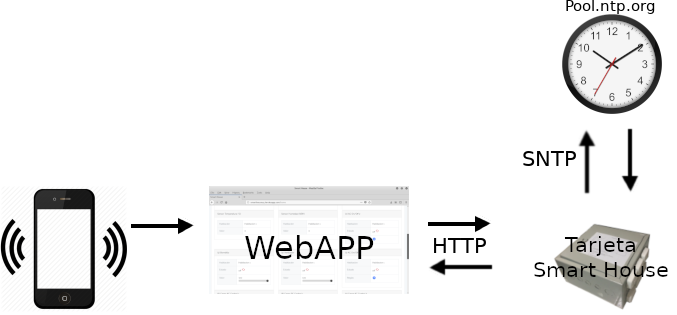
\includegraphics[width=0.5\linewidth]{Imagenes/IOT}
\end{figure}

\subsection{Software}

\subsubsection{Aplicación Web}

En la Figura \ref{fig:r-adm}\textbf{(a)} de la imagen se observan algunos dispositivos registrados en la aplicación web, el administrador puede editarlos pero no puede cambiar su estado o visualizar su valor, ya que esto es algo privado de cada dispositivo. En la Figura \ref{fig:r-adm}\textbf{(b)} se observan algunos usuarios creados y el mismo usuario administrador con sus datos y rol. Además en la Figura \ref{fig:r-room} se puede observar la habitación que se ha creado de prueba con sus correspondientes datos, nombre, descripción, usuarios y su token, el cual es muy importante para la seguridad de la comunicación entre el sistema embebido y la aplicación web.\\

\begin{figure}[!t]
	\centering
	\caption[Panel de Administrador.]{Panel de Administrador. [Imagen Propia]}
	\subfigure[Dispositivos]{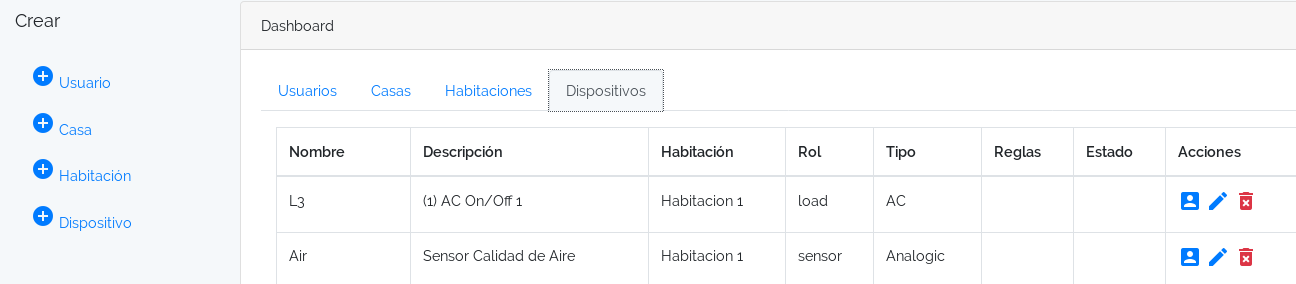
\includegraphics[width=\linewidth]{Imagenes/R_admA}}
	\subfigure[Usuarios]{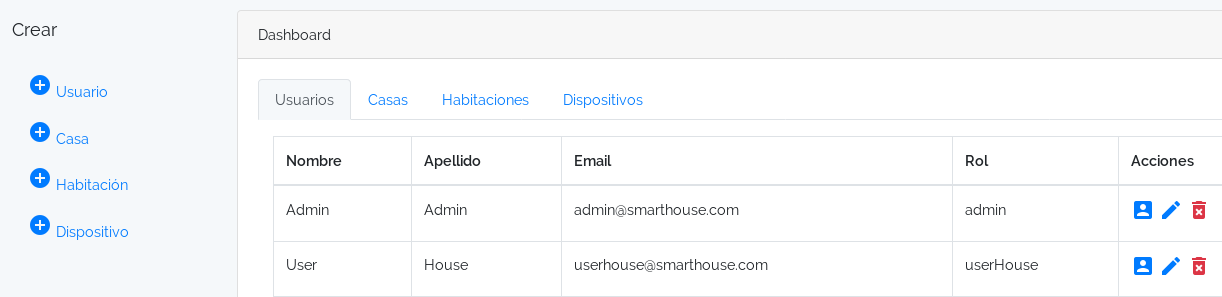
\includegraphics[width=\linewidth]{Imagenes/R_admB}}
	\label{fig:r-adm}
\end{figure}

\begin{figure}[!t]
	\centering
	\caption[Vista Habitación Usuario Administrador.]{Vista Habitación Usuario Administrador. [Imagen Propia]}
	\label{fig:r-room}
	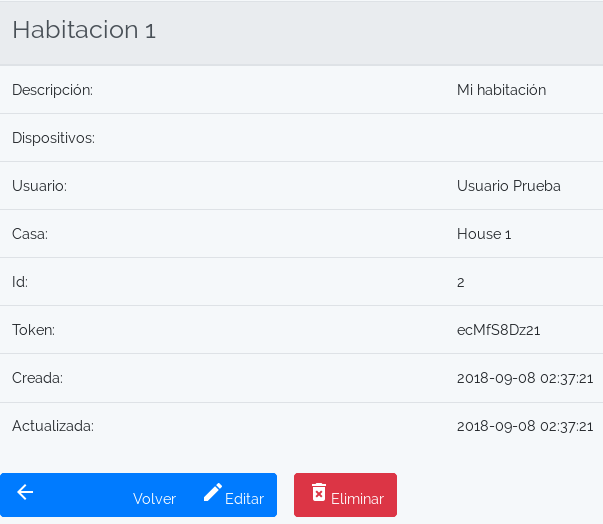
\includegraphics[width=0.45\linewidth]{Imagenes/R_room}
\end{figure}

Del mismo modo, el usuario habitación, se presenta un panel de control con todos los dispositivos presentes en su habitación denominada ``Habitación 1'', en este caso se puede observar en la Figura \ref{fig:r_app} que está el sensor de temperatura con su respectiva medida, también el bombillo y una tira LED apagada. Para encender o apagar cualquiera de estos dispositivos se presiona en el botón rojo o verde según el caso en la parte de ``Estado'', para cambiar su valor se debe utilizar el deslizador propuesto en la fila ``Valor'', al usarlo se puede variar la potencia del dispositivo.\\

\begin{figure}[!t]
	\centering
	\caption[Vista dispositivos habitación propuesta.]{Vista dispositivos habitación propuesta. [Imagen Propia]}
	\label{fig:r_app}
	\includegraphics[width=\linewidth]{Imagenes/R_app}
\end{figure}

%Cabe resaltar que cada sensor y salida se presentan en estas tarjetas y algunos con información diferente debido a su naturaleza, por ejemplo en la Figura \ref{fig:r_app1} se observa el sensor de lluvia con información de cuando detecto lluvia o dejo de detectar lluvia y también una salida DC para motor, como cuenta con inversión de giro el deslizador tiene valores entre -100 y 100, los valores negativas para que gire en un sentido y los valores positivos para el otro sentido.\\
%
%\begin{figure}[!t]
%	\centering
%	\caption[Vista dispositivos adicionales.]{Vista dispositivos adicionales. [Imagen Propia]}
%	\label{fig:r_app1}
%	\includegraphics[width=\linewidth]{Imagenes/R_app1}
%\end{figure}

Las diversas interfaces generadas en la aplicación, permiten el monitoreo, control y la interacción del usuario con el dispositivo presente en su habitación, haciendo posible el cambio de estado de las salidas y así mismo visualizar los datos producidos por los sensores. También cabe resaltar que algunas salidas tienen la posibilidad de automatizarse a través de reglas, es decir, indicarle en que momento encender o apagar cierto dispositivo que se encuentre conectado a la tarjeta como se ha mencionado. Por otra parte, todos los datos generados de la interacción del cliente con el programa se almacenan en la base de datos enlazada a dicha aplicación permitiendo una gestión adecuada de estos. \\

\subsubsection{Aplicación Sistema Embebido} 

La aplicación se encuentra compuesto, como se ha mencionado anteriormente, de tareas, en la figura \ref{fig:tareas} se observa un bosquejo del trabajo de las diferentes tareas de las que se compone este, tomando por función principal la encargada de gestionar la conexión a Wi-Fi y almacenar sus credenciales, dependiendo del estado de si están almacenadas o no, el sistema se comporta de una u otra forma.\\

\begin{figure}[!t]
	\centering
	\caption{Esquema de Tareas [Imagen Propia]}
	\label{fig:tareas}
	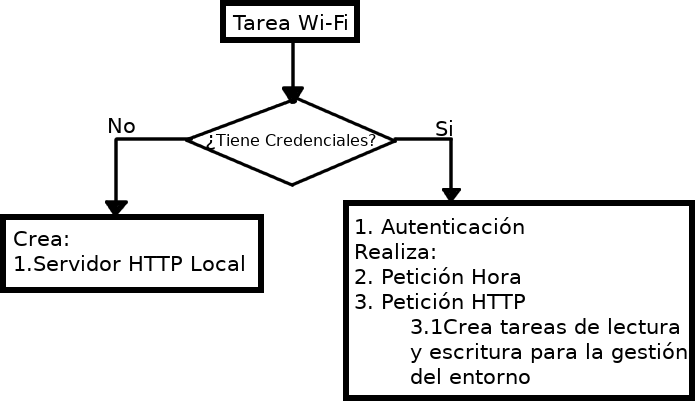
\includegraphics[width=0.7\linewidth]{Imagenes/tareas}
\end{figure}

\subsubsection*{Escritura de Datos en la Aplicación Web}

Los datos que lee la tarjeta provienen de los diferentes sensores que tiene conectados, para la escritura de estos, la aplicación dentro del ESP32 se desarrollan con varias tareas encargadas de leerlos y enviarlos a una tarea central. Como se mencionó, los datos enviados en formato JSON contienen el id del dispositivo y la medida que lee en ese momento, organizándolos en la petición HTTP tipo GET; La aplicación ya se encarga de almacenarlos y mostrarlos al usuario como se menciona anteriormente.\\

\subsubsection*{Lectura de Datos de Internet}

La tarjeta mantiene una actualización frecuente, para esto, cuando la tarjeta envía los datos de los sensores la aplicación responde con datos de respuesta HTTP, además de la información de los dispositivos que controla la tarjeta, esta los recibe en una cadena texto en formato JSON como se observa en la figura \ref{fig:httprqstesp}, los procesa y los dirige a las tareas pertinentes ya sea para encender o apagar algún dispositivo conectado a la tarjeta.\\

\begin{figure}[!t]
	\centering
	\caption{Respues del la APP Web a la Tarjeta [Imagen Propia]}
	\label{fig:httprqstesp}
	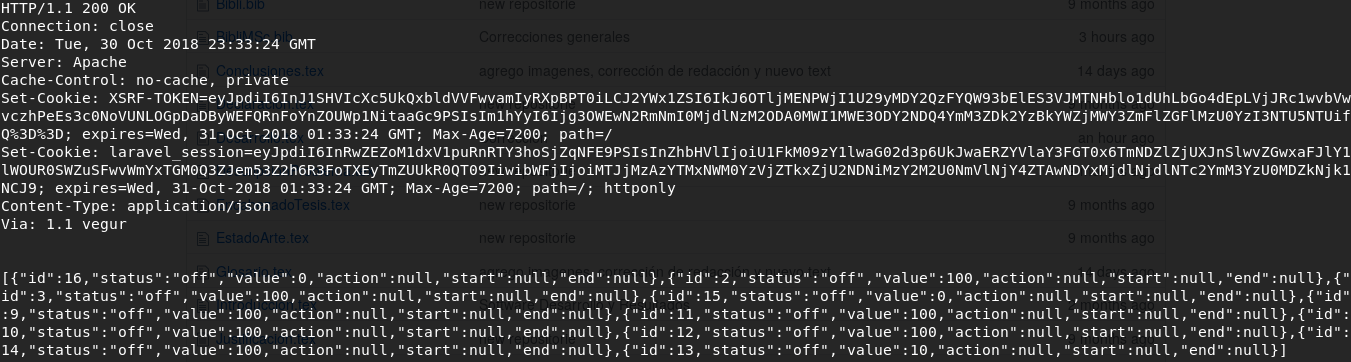
\includegraphics[width=0.9\linewidth]{Imagenes/HTTPRqstesp}
\end{figure}

Analizando los tiempos de resolución de la petición http, siempre se tiene una media de 1s el cual es un tiempo de respuesta aceptable dadas todas las funcionalidades provistas en el programa, aunque este tiempo varia, ya que se usa el puerto serie para observar estos resultados, esta comunicación agrega también tiempo al procesamiento, así que es un aproximado, asimismo interfiere la velocidad en la conexión a Internet y la señal de recepción de Wi-Fi.

\subsection{Hardware}

De acuerdo con los circuitos diseñados en la Sección \ref{sec:hw} donde se propone el desarrollo de hardware de la solución IoT, en la Figura \ref{fig:tarjeta} se observan las diferentes tarjetas ya ensambladas en una caja eléctrica para probar el funcionamiento del prototipo. Las salidas y entradas están distribuidas según lo propuesto, para las salidas AC se usan toma corrientes para conectar allí los diversos dispositivos, para las salidas DC se utilizan conectores hembra tipo banana para facilitar la conexión de estos dispositivos. La distribución de las diferentes salidas que posee la tarjeta se organizó en pegatinas y se colocaron sobre la caja eléctrica. La Figura \ref{fig:labels} muestra esta información, tanto para la parte interna como externa de la caja.\\

\begin{figure}[!t]
	\centering
	\caption[Tarjeta SmartHouse.]{Tarjeta SmartHouse. [Imagen Propia]}
	\label{fig:tarjeta}
	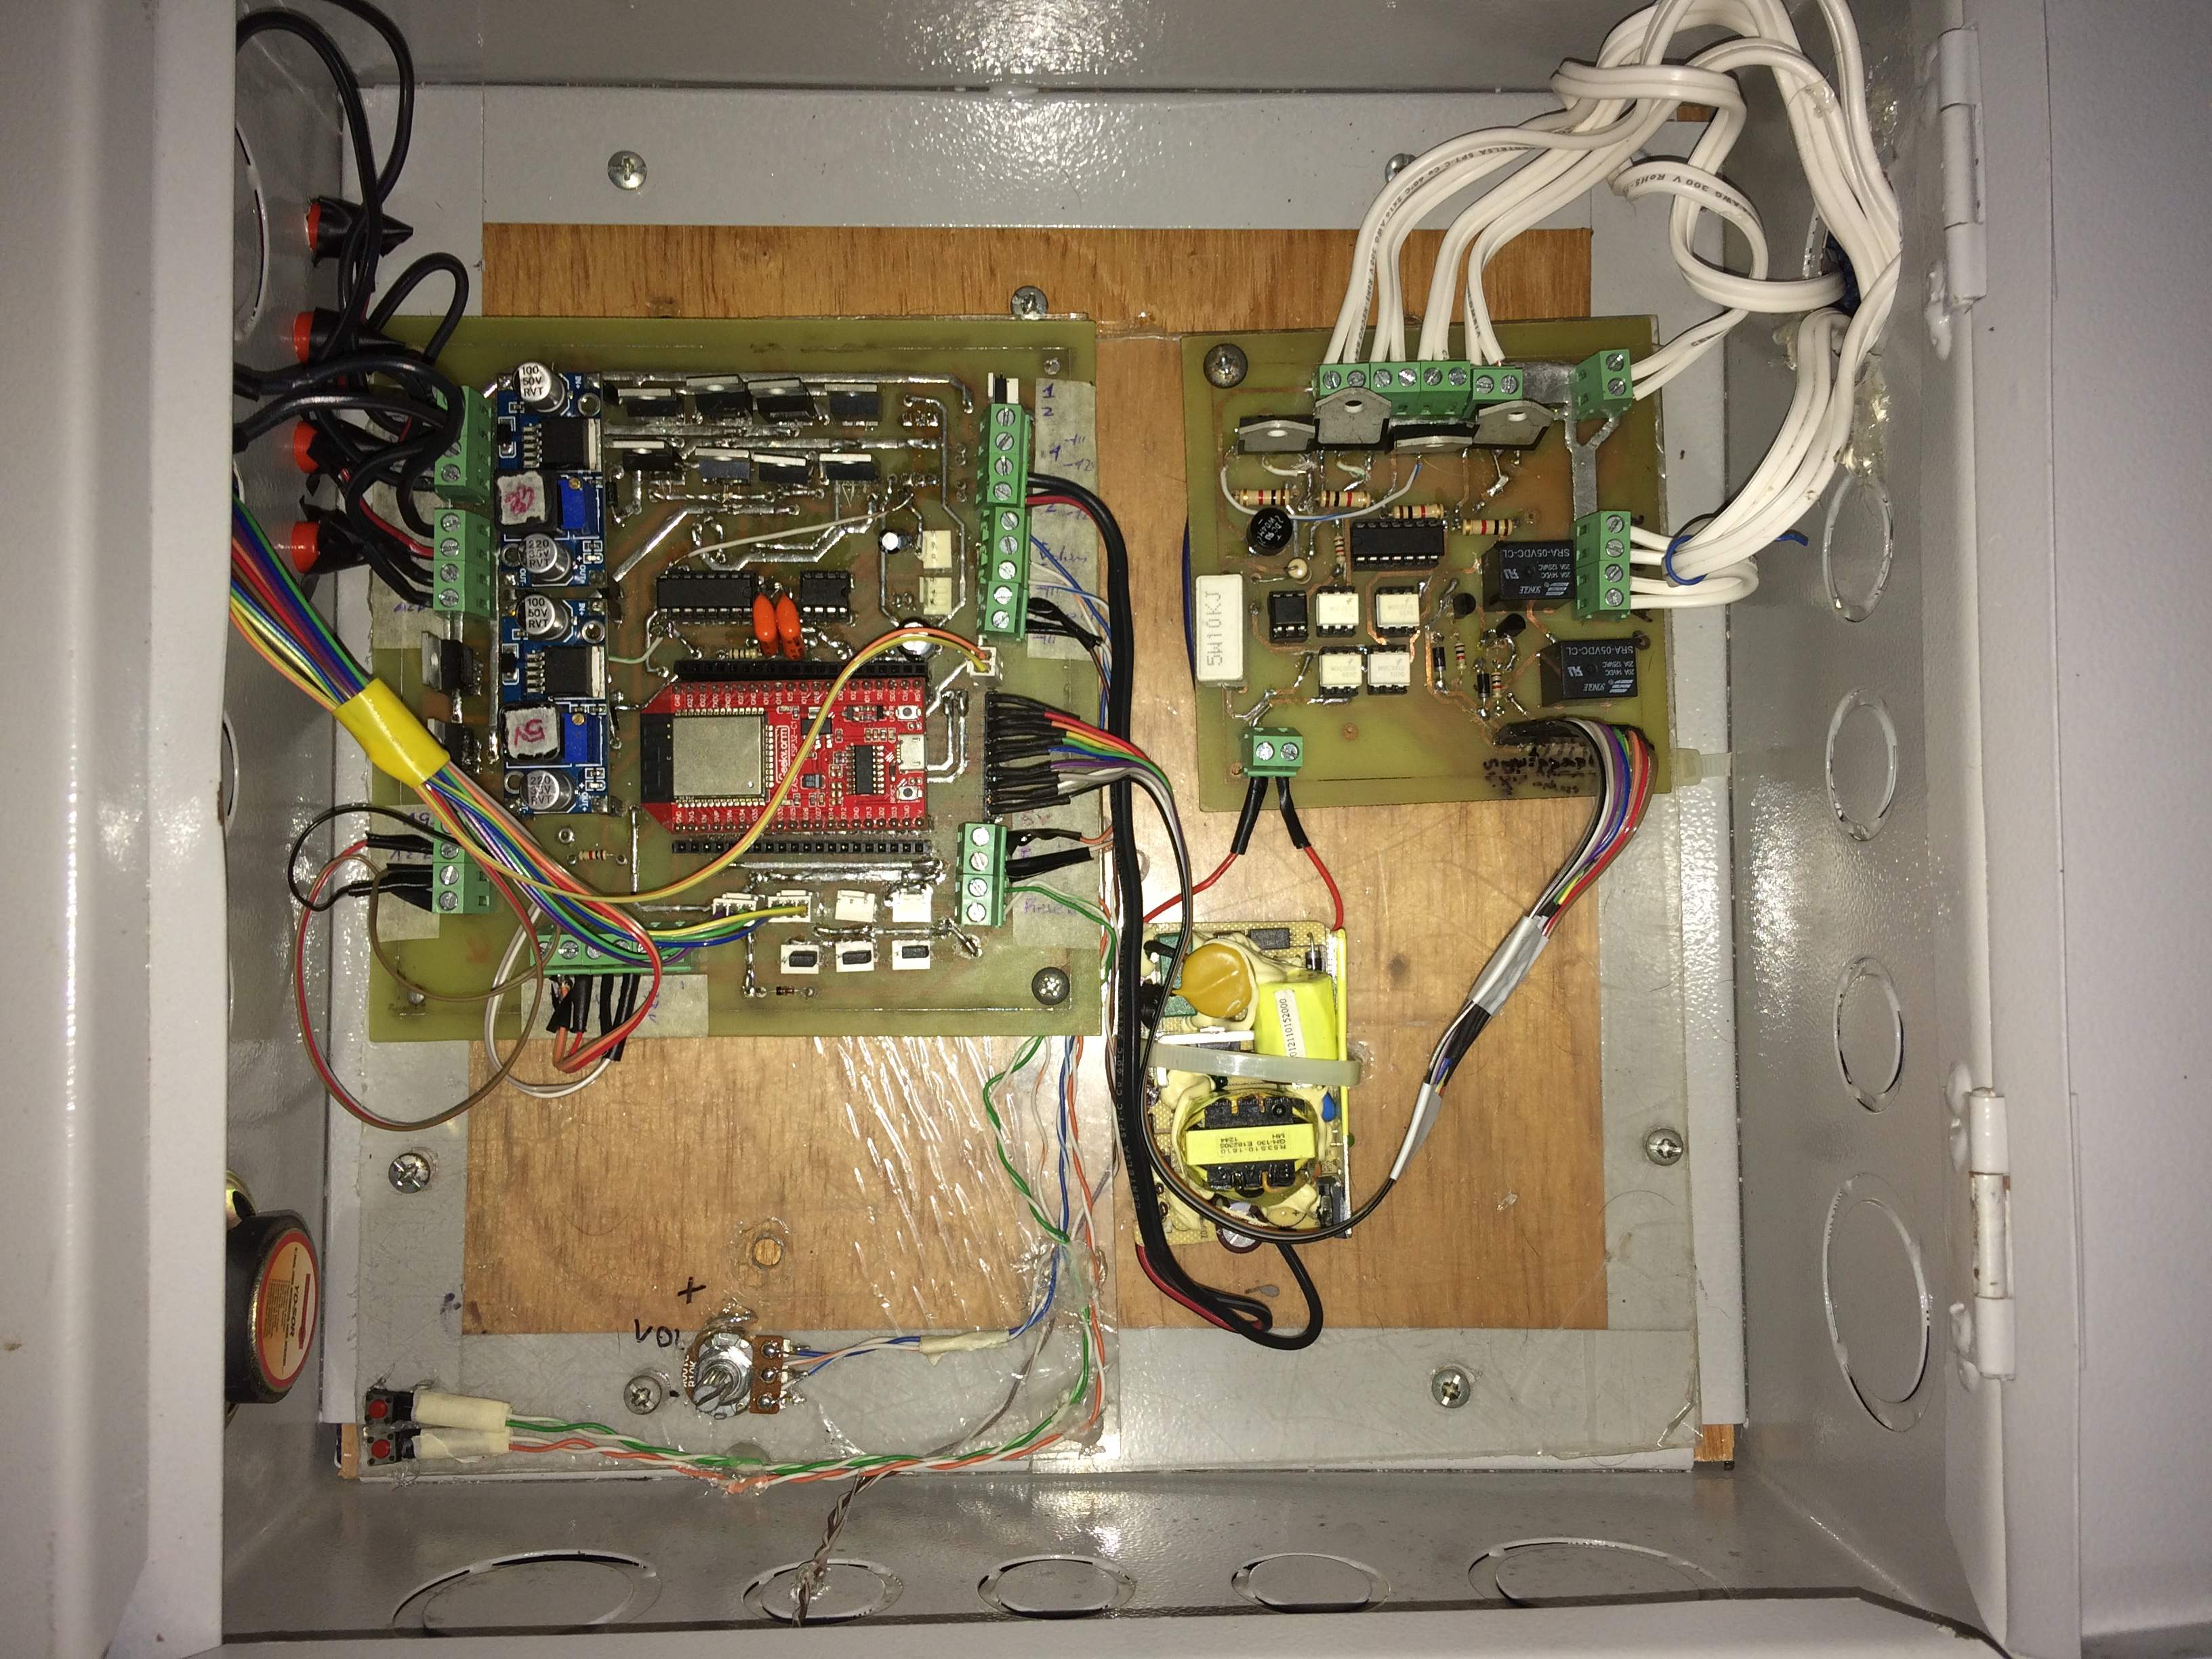
\includegraphics[width=0.6\linewidth]{Imagenes/Tarjeta.jpg}
\end{figure}

\begin{figure}
	\centering
	\caption[Descripción caja eléctrica tarjeta SmartHouse.]{Descripción caja eléctrica tarjeta SmartHouse. [Imagen Propia]}
	\label{fig:labels}
	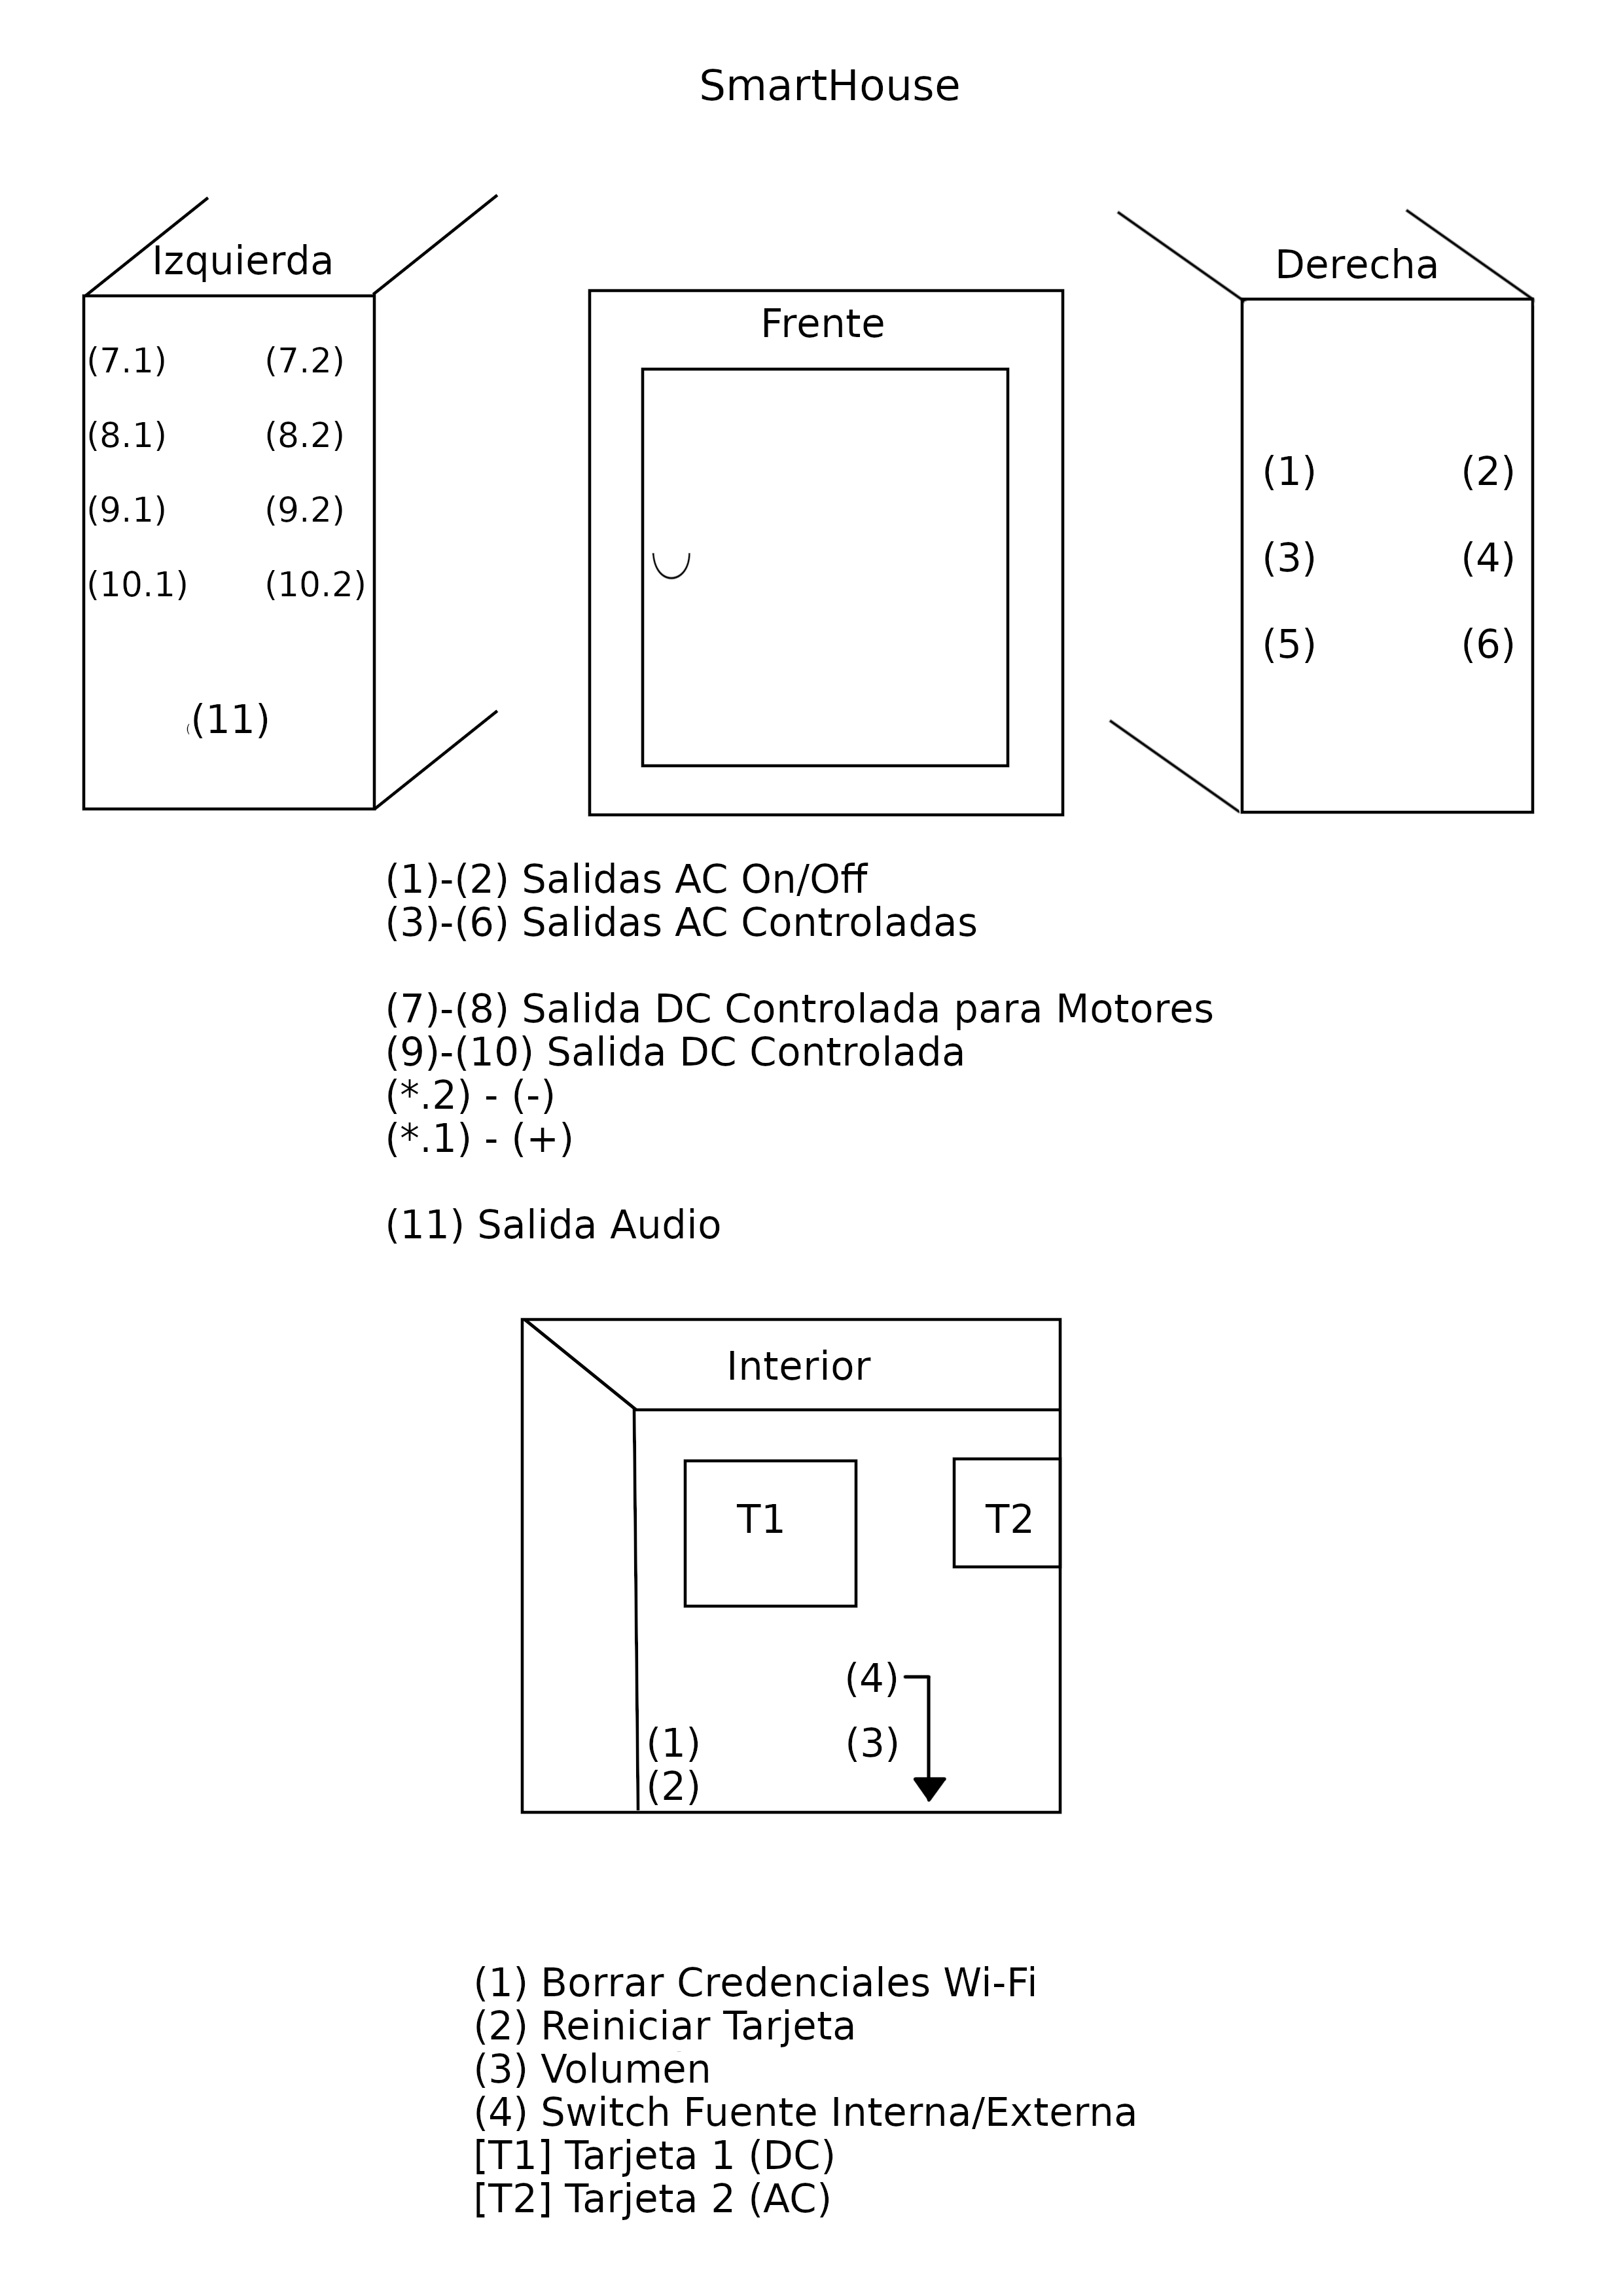
\includegraphics[width=0.7\linewidth]{Imagenes/labels}
\end{figure}

Se observa que el hardware quedo dividido en dos tarjetas, esto para facilitar la construcción y distribución de los diferentes elementos utilizados en los diferentes circuitos que componen las etapas de esta característica del sistema, de tal manera que las funcionalidades cumplen con los requisitos propuestos.\\

El sistema se ha probado con cargas AC como bombillos LED entre 7W y 20W, de filamento de 100W, probando funcionalidades como el control de potencia AC por ángulo de fase, obteniendo los resultados esperados. El voltaje de alimentación viene dado por la red eléctrica, la tarjeta simplemente conmuta el estado de la alimentación o controla la potencia entregada.\\

Para las salidas DC se realizan pruebas con un motor DC de 1W, además de una tira LED de 1W, la cual se le varía la energía entrega. Estas cargas se alimentan con 12VDC directamente desde la fuente interna o convertidor AC-DC, los circuitos que se implementan simplemente conmutan el estado de encendido/apagado o por medio de PWM variar la energía entregada.\\


\subsection{Prueba Beta Cerrada}

Esta prueba se desarrolla en el entorno del cliente o usuario, arrojando resultados sobre las funcionalidades provistas para el software, además de dar la aceptación por parte del cliente si el producto funciona de manera adecuada o esperada \cite{PB}. En general se ha propuesto el escenario de una solución IoT, con alcances como controlar cargas AC o DC y visualizar el estado del entorno de aplicación por medio de la página web desarrollada. Por este motivo se presentan los diferentes casos de prueba a realizar y se mencionan a continuación.\\

\paragraph{Prueba de conectividad de la tarjeta} La persona que participa en esta prueba debe realizar los primeros pasos para conectar la tarjeta con internet como se expone más adelante en resultados y se explica en Anexos en el manual de usuario. De acuerdo con esto se califica la forma en que el cliente realiza este procedimiento, con la finalidad de analizar si es adecuada la manera en que se conecta la tarjeta SmartHouse a Internet por medio de Wi-Fi y también como reiniciar la conexión de la tarjeta para configurar nuevamente la red a la que se va a conectar. Las preguntas que califican esta funcionalidad se mencionan a continuación:

\begin{itemize}
\item El método para conectar la tarjeta a Internet por medio de Wi-Fi es sencillo de realizar.
\item La interfaz para seleccionar la red e ingresar las credenciales es fácil de utilizar.
\item En caso del cambio de nombre o contraseña de su red Wi-Fi, es fácil volver a configurar la tarjeta para que esta se conecte de nuevo.
\end{itemize}

\paragraph{Prueba de la Aplicación Web} Evalúa el inicio de sesión, el monitoreo y control de todos los dispositivos que se encuentra conectados en tarjeta SmartHouse, además de las funcionalidades que posee el sistema en general. Para esta prueba se deben realizar diferentes procedimientos, como iniciar sesión en la aplicación, encender o apagar un dispositivo, visualizar los datos de los sensores y configurar las reglas para los dispositivos. Las preguntas presentadas a continuación califican estos aspectos y funcionalidades:\\

\begin{itemize}
	\item El inicio de sesión en la pagina web es claro.
	\item En la aplicación web, los datos de los sensores y estados de las salidas se presentan de una manera clara y entendible.
	\item Encender o apagar un dispositivo o salida es sencillo y se presenta de forma clara.
	\item El tiempo de respuesta después de encender o apagar un dispositivo desde la aplicación es bueno.
	\item Las reglas para los dispositivos o salidas son fáciles de configurar y eliminar.
	\item La aplicación web es fácil de usar.
\end{itemize}

Al ser una prueba beta cerrada el desarrollador escoge un número de personas determinadas con distintas características, por este motivo se realiza a quince personas, entre los cuales algunos son estudiantes de ingeniería electrónica, estudiantes de otras carreras, profesionales y personas ajenas a este tipo de escenarios, los resultados de la prueba se consignan en la Tabla \ref{table:enc}. Estas personas interactúan directamente con la aplicación web y el prototipo de la tarjeta SmartHouse. para evaluar las características mencionadas se califican de acuerdo con una escala tipo likert \cite{lik} de uno a cinco en la cual, cinco es la calificación máxima y uno la mínima.\\


\begin{table}
	\begin{center}
		\caption{Resultados por pregunta.}
		\label{table:enc}
		\begin{tabular}{|c|c|}
			\hline 
			\textbf{Número de la Pregunta} & \textbf{Promedio} \\ 
			\hline 
			1 & 4.5\\ 
			\hline 
			2 & 4.8\\ 
			\hline 
			3 & 4.5\\ 
			\hline 
			4 & 5.0\\ 
			\hline 
			5 & 4.9\\ 
			\hline 
			6 & 4.9\\ 
			\hline 
			7 & 4.3\\ 
			\hline 
			8 & 4.3\\ 
			\hline 
			9 & 4.8\\ 
			\hline 
			\textbf{Total} & \textbf{4.7}\\ 
			\hline 
		\end{tabular} 
	\end{center}
\end{table}

En resumen, el sistema recibe una calificación de 4.7, por lo tanto se puede decir que las funcionalidades requeridas están programadas de una manera adecuada y simple para que el usuario disponga de ellas, pero es posible mejorarlas con el objetivo de que sean mucho más intuitivas para el usuario y que no se le presenten dudas al momento de usarla. Conforme a las observaciones obtenidas durante la prueba se han modificado algunas partes del sistema, que no tienen un impacto significativo sobre los objetivos ni alcances propuestos en este trabajo.\\

Algunas características importantes resultantes de la prueba, recaen en la organización del hardware, de tal manera que sea más intuitiva la conexión y la manipulación de los botones, los cuales requieren un posicionamiento visualmente más cómodo dentro de la caja eléctrica en la que se encuentra el sistema. Por otra parte, el manual requiere modificaciones en la explicación de algunos procesos, ya que a pesar de que este permite el manejo correcto del sistema, requiere mayor detalle en procedimientos que requieren conocer aspectos como el manejo de un dispositivo inteligente o claridad adicional al usar el dispositivo por primera vez.\\

Además de esto, es importante resaltar que las interacciones de los usuarios a través de la aplicación web se realizan de manera fácil y entendible, pues los aspectos relacionados con esta y su navegación, mantienen el promedio más alto de la prueba, dejando claro que este aspecto del sistema tuvo gran éxito en cuanto a los usuarios se refiere.\\